\begin{exercise}{Fibre$\cdot$s optique$\cdot$s}{2}{Sup}
{Réfraction, Optique géométrique}{bermudez}

On étudie la propagation d'un faisceau lumineux d'incidence $i$ dans une fibre optique formée d’une âme d’indice $n_\text{a} = 1,66$ et de rayon $r = 1$ mm entourée d’une gaine en verre d’indice $n_\text{g} = 1,52$.

\begin{figure}[H]
\centering
    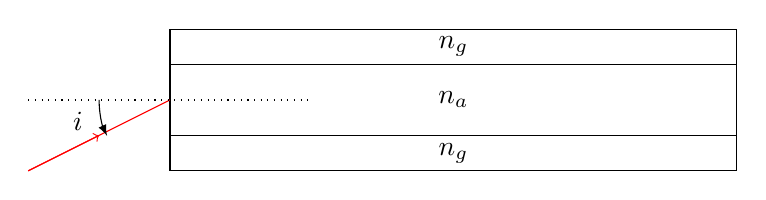
\begin{tikzpicture}[scale=.9] 
%fibre optique 
\draw (0,0) --+ (8,0); 
\draw (0,-0.5) --+ (8,0); 
\draw (0,-1.5) --+ (8,0); 
\draw (0,-2) --+ (8,0); 
\draw (0,0) --+ (0,-2); 
\draw (8,0) --+ (0,-2); 
%\draw [->,color=red] (0,-1) --++ (2,0.5) --++ (4,-1) --++ (4,1) --++ (4,-1) --++ (1,0.25); 
\draw [color=red] (0,-1) --++ (-2,-1); 
\draw [->,color=red] (-2,-2) --++ (1,0.5); 
\node at (4,-0.25) {$n_\text{g}$}; 
\node at (4,-1.75) {$n_\text{g}$}; 
\node at (4,-1) {$n_\text{a}$}; 
\draw [dotted](-2,-1)--++(4,0); 
\draw [->,>=latex] (-1,-1) arc (0:25:-1.2); 
\node () at (-1.3,-1.3) {$i$}; 
\end{tikzpicture}
\end{figure}

\begin{questions}
    \questioncours Démontrer la relation de Snell--Descartes à partir du principe de Fermat.
    \question \textsf{Culture sciences--physiques :} Applications de la fibre optique. Avantages et incovéniants.
    \question Quelle l'incidence maximale $i_\text{max}$ sous laquelle le rayon est entièrement réfléchi ? On exprimera l'ouverture numérique de la fibre $\text{ON} \equiv \sin i$ en fonction des indices de la fibre.
    \question On veut se servir d'une telle fibre, sans la gaine, pour détecter la présence d'eau ($n_\text{e} = 1,33$) ou d'air (considéré comme du vide d'indice 1) dans un réservoir.
    Proposer une valeur de l'incidence pour mettre en place ce dispositif.
    
    \question Évaluer le retard $\tau$ entre l'entrée et la sortie de $L = 1$ km de fibre sous incidence $i = 8^\circ$.
    \question Une fibre réelle atténue le signal à cause de l'absorption et de la diffusion de la lumière par le matériau. Pour $\lambda = 800$ nm, on a
    $$A = 10\log(I_\text{in}/I_\text{out}) = 1,2 \mathrm{ dB\cdot km^{-1}}.$$
    Au bout de combien de kilomètres restera-t-il 10\% du flux incident ?
    
    \question On suppose l'incidence nulle, mais que la fibre est courbée avec un rayon de courbure $R = 10$ cm. Calculer l'incidence $i'$ du rayon arrivant à l'interface gaine--âme et donner une condition sur $r$ et $R$ pour que le rayon soit totalement réfléchi.
\end{questions}

\end{exercise}
